\documentclass[../MaxHughesThesis.tex]{subfiles}

\begin{document}

The experiment was run at the National Superconducting Cyclotron Laboratory (NSCL) in East Lansing, Michigan from September 1, 2015 to September 7, 2015.
The experimental technique avoids many of the systematic effects that were important in previous shape measurements in  $^{20}$F.

\section{Experimental Technique}
The technique used was a calorimetric technique, where the isotope of interest is implanted inside a detector.
This reduced several effects that could otherwise distort the beta energy spectrum.

With the calorimetric technique, the radioactive nucleus is surrounded by detector material.
As long as the nuclei are implanted deep enough, the electrons will not have enough energy to escape the detector.
Even if the electron scatters several times, it still deposits all its energy.
This range depends on the detector material.
Since any dead layers are at the surface, the decays inside the detector do not see them.
A $4\pi$ angular coverage is also obtained, as the detector material surrounds the source completely.

There are some caveats for a calorimetric technique. 
The first is that a large enough detector is needed, since otherwise the electrons could escape at high energies.
A large effect is that electrons moving through the detector material will emit a lot of bremsstrahlung.
Using a low-$Z$ detector material will lessen this effect.
However, Monte Carlo detector simulations can describe the production and absorption of bremsstrahlung well enough to allow for a precision beta spectrum measurement \cite{Huy18}. 
Another issue is that accelerators used to generate the isotope of interest must be able to create them at high enough energy in order to implant the isotopes deep enough into the detector.
This limits what nuclei can be used for this technique.
The act of implanting the nuclei gives the detector a lot of energy. 
This means that an implant and decay cycle is needed for this experimental technique.

For this experiment, a  beam of  $^{20}$F, was implanted into two different detectors, which were used to cross-check different systematic effects.
One was a CsI(Na) scintillator detector, and the other was a  EJ-200 polyvinyltoluene (PVT) scintillator detector. 
After an amount of $^{20}$F was implanted, the beam was turned off by dephasing the RF that drove the cyclotrons.
Then, the $^{20}$F was allowed to decay inside the detector. 
Given the half-life of $^{20}$F of 11 s, the measuring time was varied between 22 and 60 s.

\section{The $^{20}$F Beam}

The beam of $^{20}$F was created at the coupled cyclotron facility at the NSCL.
The primary beam of $^{22}$Ne was accelerated by the coupled cyclotrons to 150 MeV/A. 
A typical intensity of the primary beam was around $60 \times 10^{-5}$ pnA.
It was impinged on a 188 mg/cm$^{2}$ Be target and sent through the A1900 fragment separator. 
The resulting $^{20}$F beam was at an energy of 130 MeV/A. 
The intensity of the $^{20}$F was about $2 \times 10^{-5}$ pnA.
The beam was sent to the experimental vault were the detectors were sitting.

\subsection{Beam Size and Location}
\label{sec:beamsize}
To test the size of the beam, a parallel plate avalanche counter (PPAC) was used.
The size of the detector was 10 cm by 10 cm square. 
It was placed 65 cm upstream of the detector.
A horizontal and vertical grid was in the detector.
Depending on where on each of the grids the particles hit, different charges were sent to either end of the PPAC.
The signals were fed into a digital data acquisition system, and read out as an energy.
The difference of the two signals divided by the sum was interpreted as a position.
The location of the PPAC and other detectors are shown in figure \ref{fig:BeamSetUp}.

\begin{figure}
	\centerline{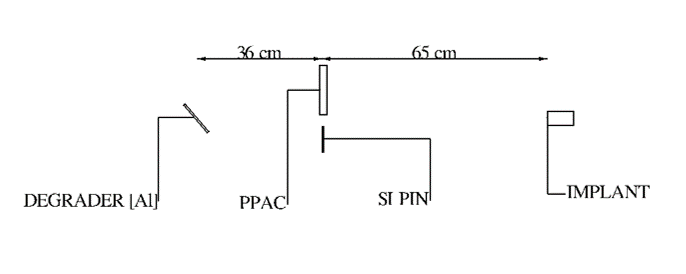
\includegraphics[width=0.88\textwidth]{ScaleOfBeamLine_v2.png}}
	\caption{A sketch of the location of the detectors upstream of the implant detector.
		    The detectors are not to scale. 
			}
	\label{fig:BeamSetUp}
\end{figure}  

To calibrate the PPAC, a mask with several holes was used. 
This mask covered the front of the detector, and an alpha decay source in the vacuum was placed in front of the PPAC.
Then, everything was left to run until an image of the mask was formed.
The mask had holes in it every 1 cm. 
It also had a large L shaped hole so that the orientation of the mask could be seen. 
With this, the PPAC could be calibrated.

Before taking data for the beta energy spectrum measurement, the PPAC was inserted into the beam.
After adjusting the parameters of the upstream beam optics, the final beam size at the PPAC was measured.
The calibrated data of the signals was built into a 2-D histogram.
There was some ringing in the PPAC.
To suppress this ringing, a threshold for the PPAC was applied. 
To calculate the threshold, the peak of the beam spot was fit with a 2-D Gaussian function
The centroid of the Gaussian and the sigma in the $x$ and $y$ direction was taken. 
From the standard deviations, the half widths at half maximum (HWHM) in both directions were calculated. 
Using the HWHM and the center of the Gaussian, 8 points were selected.
These eight points are the black dots in figure \ref{fig:PPACSpotch}.
The $z$ values of the PPAC distribution at each of those points was averaged.
This value was the threshold above which the PPAC distribution was plotted.  
The resulting width was read off to be 8 $\times$ 6 mm.

\begin{figure}
	\centerline{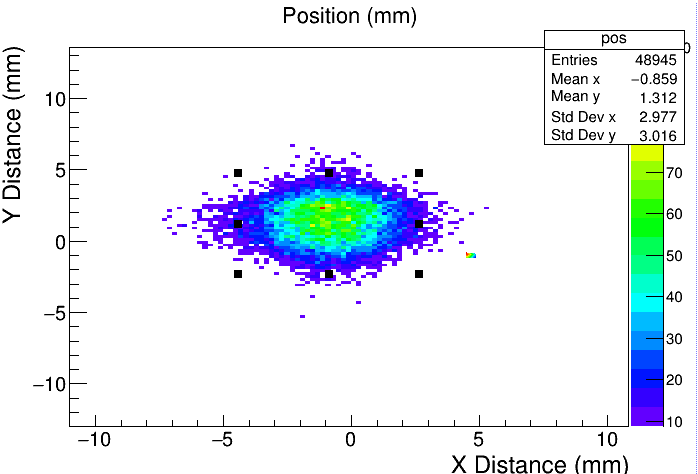
\includegraphics[width=0.74\textwidth]{PPACFitted.png}}
	\caption{The beam spot of the calibrated PPAC spectrum. 
		 The samples of the spectrum that were averaged together are shown in the black dots.
		 The center of the fit is not shown.}
	\label{fig:PPACSpotch}
\end{figure}  

This is the size of the spot at the location of the PPAC. 
Ion optics simulations were used to build the envelope of the beam at the PPAC and at the target.
Using these cross sections, the magnification between the two locations was calculated.
The magnification was different for the $x$ and $y$ directions.
With these magnifications, the beam spot at the stopping position was deduced to be 3.6 $\times$ 3.5 mm.  

For the depth of the implantation of the beam, ion simulations were used. 
The LISE++ program was fed the geometry and the settings of the beam magnets. 
It was given the energy of the beam and the location of the implant detector. 
It then calculated the depth of the implantation in the detector and the range of the depth inside the detector. 
This gave a depth of 3.02 cm in side the PVT detector and a depth of 1.156 cm in the CsI(Na) detector. 
The range straggling was 1.2 mm in the PVT detector and 0.4 mm in the CsI(Na) detector.

\subsubsection{Verification of Implantation Depth}

In order to verify the simulations for the beam implantation depth, a degrader was inserted into the beam for a beam depth measurement, which is shown in figure \ref{fig:degraderdata}.
The degrader was made of aluminum and had two different thicknesses: 7.89 mm and 11.38 mm. 
The beam was caught by a CsI(Na) scintillator of a similar design to the one used during the main measurement.
The angle of the degrader was changed to change the effective thickness of aluminum that the beam had to travel through. 
By comparing the measurement to the one predicted to stop the beam outside of the detector, the depth of implantation could be verified. 
This was done after the main run, and the simulation matched the measurement.
The two are plotted side by side in figure \ref{fig:degraderdata}.

\begin{figure}
    \centering
    \begin{minipage}{0.50\textwidth}
	\centerline{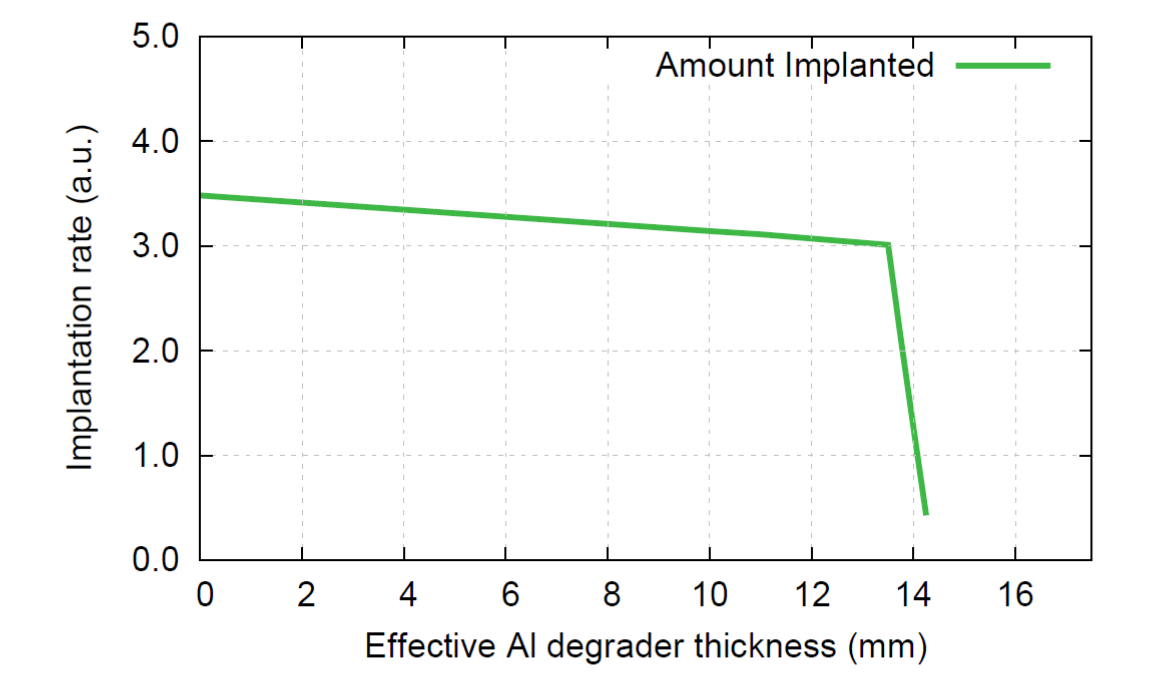
\includegraphics[width=0.90\textwidth, height = 4 cm]{degrad.png}}
    \end{minipage}\hfill
    \begin{minipage}{0.50\textwidth}
	\centerline{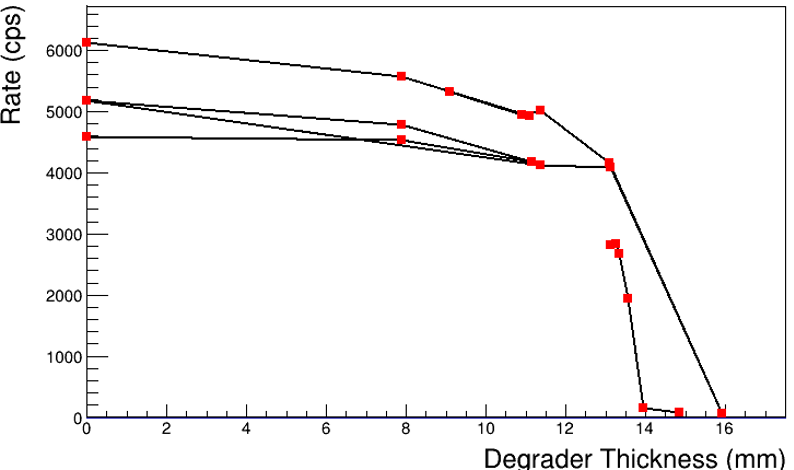
\includegraphics[width=0.90\textwidth, height = 4 cm]{CsIDegvRateWithLines_Cropped.png}}
    \end{minipage}
	\caption{The simulation is on the left.
		 The data is on the right.
		 All the fluorine is blocked after 14 mm of degrader.}
	\label{fig:degraderdata}
\end{figure}


\section{Detector Configuration}

\subsection{Detectors}
One implant detector was a scintillator 3"\diameter $\times$  3 " cylinder of EJ-200 polyvinyltoluene (PVT).
It was glued to a clear acrylic disk glued to a photomultiplier tube.
The plastic detector signal is fast (around 10 ns wide) which makes pile-up a lesser concern.
This detector was built by collaborators from Wittenburg University.
During the experiment, the voltage on the PMT of this scintillator was varied and a gain monitoring system was installed.

To monitor the gain of the plastic detector, an acrylic disk containing an optical fiber was placed between the crystal and the photomultiplier tube. 
The other end of the fiber was fed into a box with a LED driven by a function generator, which ran at a trigger rate of 500 counts per second. 
The function generator produced two pulses separated by 136 $\mu$s.
These two pulses had different amplitudes, so that the gain drift could be monitored by observing the drift from two different energies.
The box was made light-tight with electrical tape and black paint.
An additional optical fiber fed the light to a Si PIN diode.
This was to monitor the light output of the LED.
A sketch of the PVT scintillator including the acrylic disk is shown in figure \ref{fig:PVTDetSketch}.

\begin{figure}
	\centerline{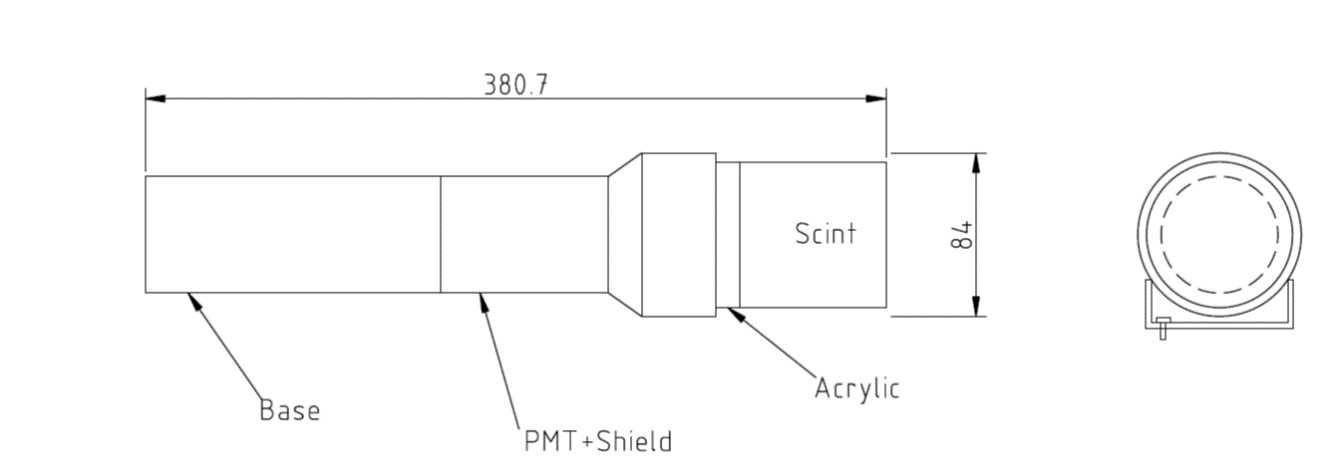
\includegraphics[width=0.90\textwidth]{PVTDetectorSketch.png}}
	\caption{A sketch of the PVT implant detector.
		    The acrylic disk is seen along as PVT scintillator. 
		   }
	\label{fig:PVTDetSketch}
\end{figure}
To check for systematics effects, another implant detector was used.
It was a 2" $\times$ 2" $\times$ 4"  CsI(Na) detector. 
This detector was a module from the CAESAR array \cite{Wei10}.
It does not have any gain monitoring like the PVT detector.

In order to measure the gamma ray from the $^{20}$F decay, a frame was built to hold four 3" $\times$ 3" $\times$ 3" CsI(Na) detectors.  
These were also part of the CAESAR array.
The frame to hold the four detectors was designed to be able to move the four outer detectors around.
A sketch of the PVT implant detector configuration is shown in figure \ref{fig:detsketch}.
A sketch of the CsI Implant detector configuration is shown in figure \ref{fig:csiimdetsketch}.

\begin{figure}
	\centerline{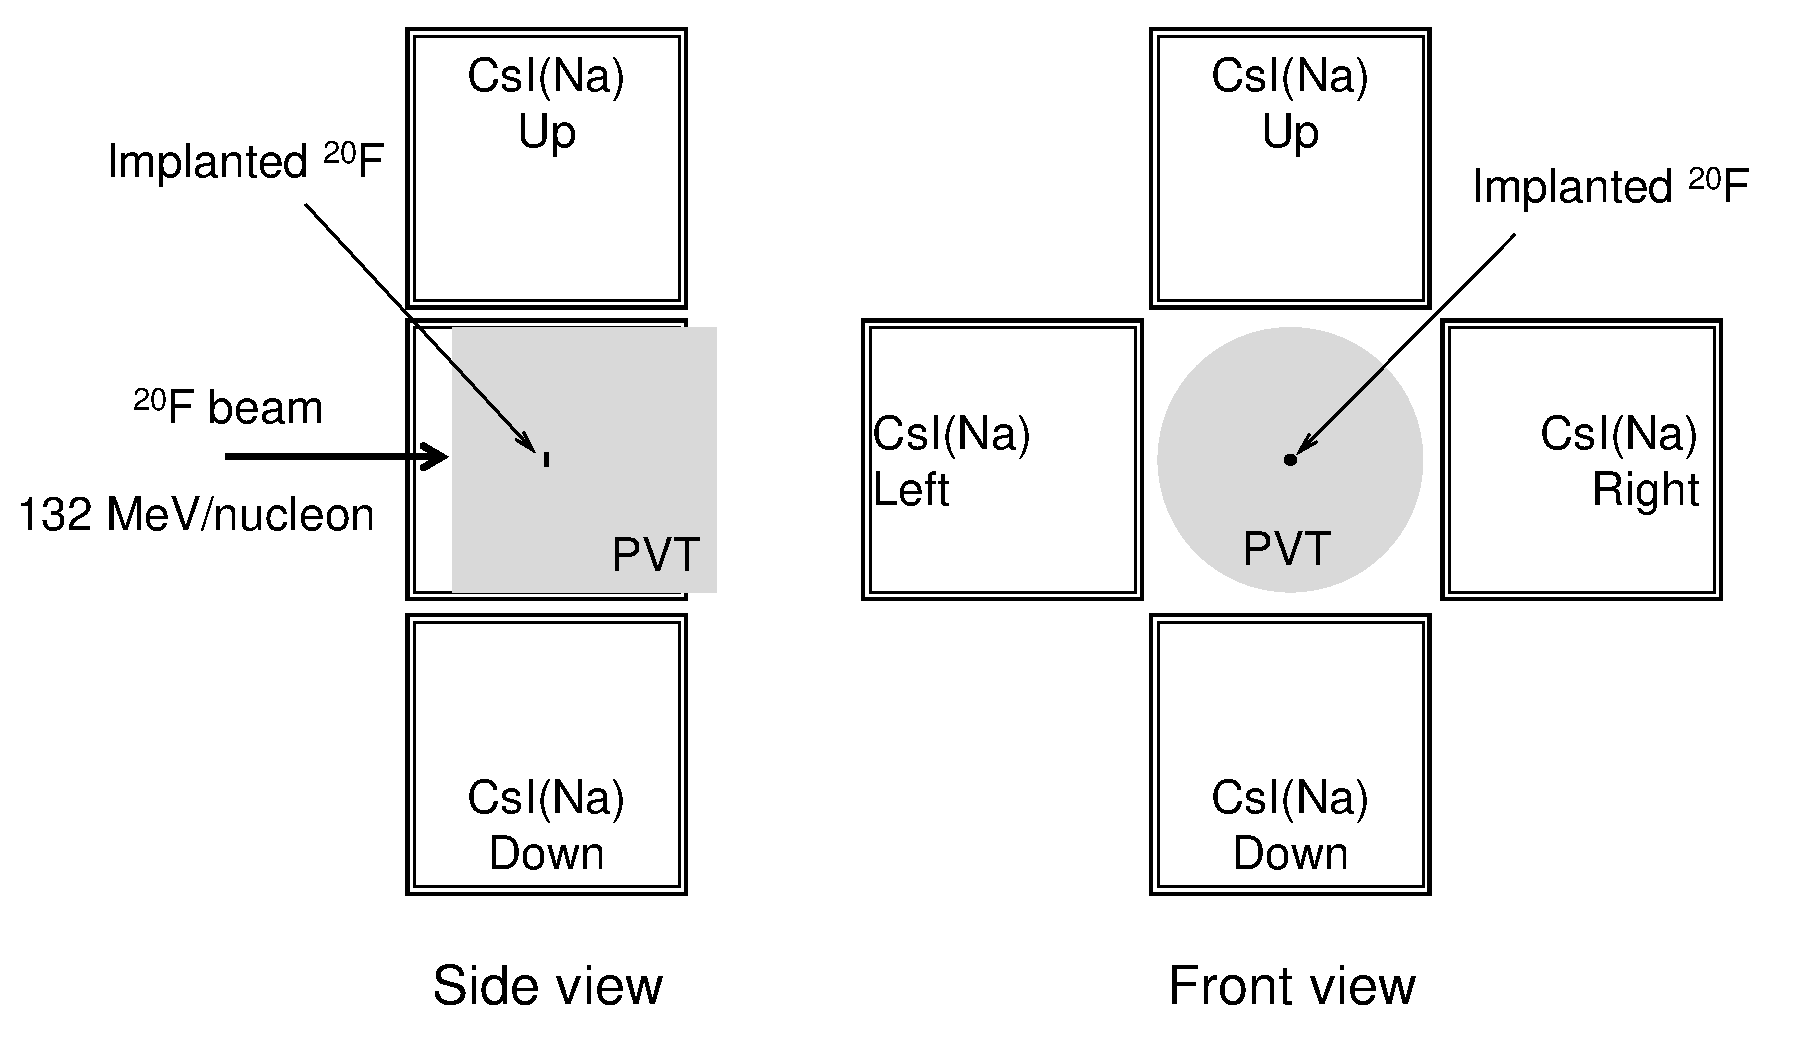
\includegraphics[width=0.68\textwidth]{fig_setup.pdf}}
	\caption{A sketch of the PVT implant detector set up. 
		 Notice that the PVT detector fills up the space between the gamma detectors.
		 }
	\label{fig:detsketch}
\end{figure}

\begin{figure}
	\centerline{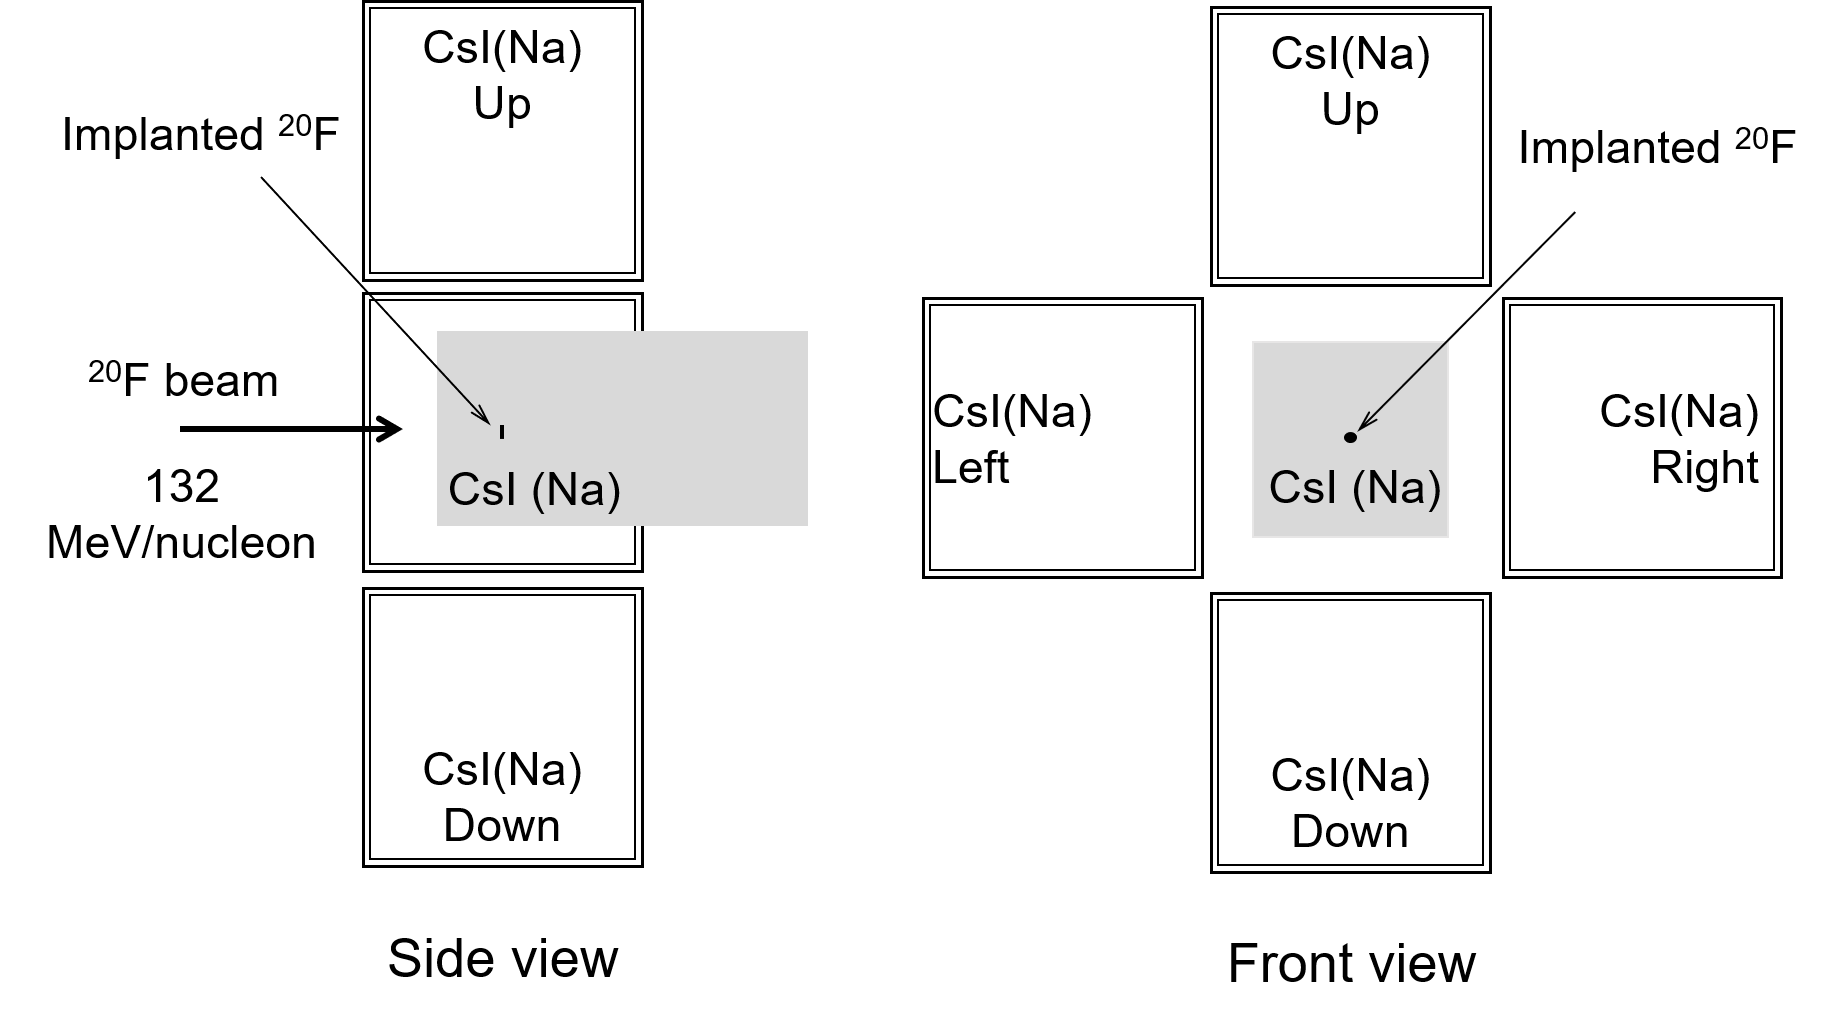
\includegraphics[width=0.68\textwidth]{fig_CsINaImplantSketch.png}}
	\caption{A sketch of the CsI(Na) implant detector set up. 
		    The CsI(Na) detector is recessed 1 inch. 
			}
	\label{fig:csiimdetsketch}
\end{figure}
To switch between different implant detectors, the central detector in the frame was removed and put on the floor.
The other detector was placed in the center of the four gamma detectors.
The PVT detector was supported on a metal rail, while the CsI (Na) detector was supported on pile of scrap aluminum.
Pictures of both detector set ups can be see in figure \ref{fig:PVTPicture}.

\begin{figure}
    \centering
    \begin{minipage}{0.50\textwidth}
	\centerline{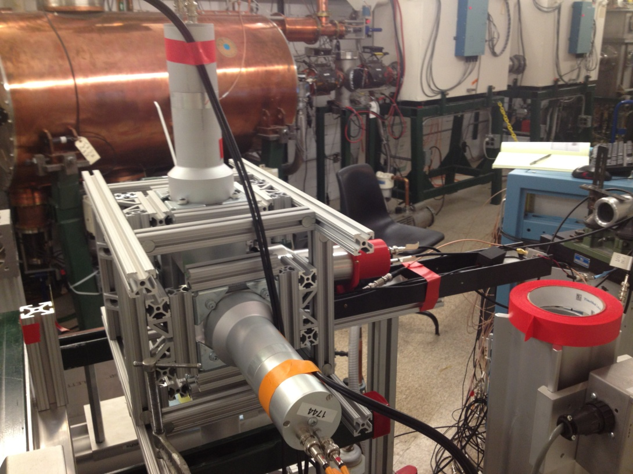
\includegraphics[width=0.90\textwidth]{fig_PVTSetupPicture.png}}
    \end{minipage}\hfill
    \begin{minipage}{0.50\textwidth}
	\centerline{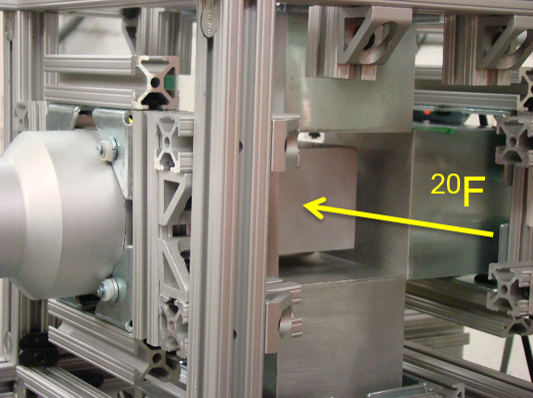
\includegraphics[width=0.90\textwidth]{fig_CsISetupPicture.png}}
    \end{minipage}
	\caption{On the left the PVT set up can be seen. 
		 The rail the detector sits on and the optical fibers (the black cords) can be seen.
		 On the right the CsI(Na) set up can be seen.
		 In the center the implantation detector is seen.
		 }
	\label{fig:PVTPicture}
\end{figure}

\subsection{Powering the Detectors}

To power the gamma and implant scintillators, three 2-channel NHQ 212M ISEG power supplies were used.
The Si detector was powered by a Tennelec TC248 amplifier.
The PPAC was powered by an integrated power supply.

Each detector had a different voltage. 
The PVT implant detector was varied in voltage over the course of the experiment.
Initially, the high voltage on the PVT detector was chosen to take advantage of the dynamic range of the detector.
Due to concerns about the beta energy spectrum shape, the voltage on the PVT detector was changed to several values as the experiment went on. 
For the PPAC, the voltage setting was adjusted to get a large enough signal.
The voltage for the four gamma detectors was chosen so that they had roughly the same gain.
The voltages of the detectors is shown in table \ref{tab:detvolt}.
\begin{table}[!hbt]
	\caption{Detector voltages.}
	\centering
		\begin{tabular}{lr}
		Detector & Power Supply Setting (V) \\ \hline
		PVT Implant Setting 1 & -975 \\
		PVT Implant Setting 2 & -856 \\
		PVT Implant Setting 3 & -780 \\
		CsI (Na) Implant & 780 \\ 
		CsI (Na) Gamma 1 & 930 \\
		CsI (Na) Gamma 2 & 1000 \\
		CsI (Na) Gamma 3 & 970 \\
		CsI (Na) Gamma 4 & 1015 \\
		Si Pin & 20 \\
		Pin diode & 15 \\
		PPAC & 560  
		\end{tabular}
	\label{tab:detvolt}
\end{table}

During the implantation cycle, a large amount of current was generated in the implant detectors.
In order to counteract this, a limiter box was installed.
The limiter box had several relays that reduced power to the PVT detector's photomultiplier tube during the beam-on cycle. 
To accomplish this, the limiter box was given the same signal that fed the beam-on/beam-off for the cyclotrons.
For the CsI(Na) implant detector, the HV supply had the current limiter enabled.
The power setting was not changed for the CsI(Na) implant detector. 


\section{Experimental Conditions}
The data was taken in runs of roughly one hour. 
However, many runs where cut short when the DAQ stopped recording data for one of the detectors.
This was usually the up gamma detector, and was correlated with the start of a new implant cycle.
In order to properly measure the decay, the beam was pulsed with an implantation time of anywhere from 1 to 2 seconds, and a decay time ranging from 22 s to 32 s. 
The beam was turned off since the light from the implantation of the beam would drown out any signal obtained. 
A run with a decay time of 60 seconds was also taken for each implant detector. 

To achieve the beam pulsing, two timer boxes were used.
A CAEN N1145 quad scaler module was used to control the beam-off time.
This module had a digital control of time down to 1 ms.
Once the the time finished counting down, a signal was sent to a second module. 
A CAEN N93B dual timer used the signal from the quad scaler as a start signal.
The beam-on time period was set with an oscilloscope, which was less precise. 
Once the dual timer finished its time, it sent a signal back to the quad scaler to restart the cycle.
The output of these two modules created a signal with one voltage level during the dual timer's time and another voltage condition during the quad scaler's time.
This signal was fed into a box.
The voltage level during the quad scaler's time dephased the cyclotron RF, turning the beam-off.
When the dual timer voltage level occurred, the RF returned to the tuned value, turning the beam-on.  
A flowchart showing the timing circuit is shown in figure \ref{fig:TimingFig} 
\begin{figure}
	\centerline{
\includegraphics[width=0.68\textwidth]{BeamOnBeamOffFigure_v2.png}}
	\caption{The modules used for the timing.
		 "Disc" stands for discriminators.
		 }
	\label{fig:TimingFig}
\end{figure}
\end{document}
